\Section{Архитектуры компьютерных сетей}{Лекция 1}{Игорь Смирнов}

\Subsection{Эталонная модель ISO/OSI}

Компьютерные сети существуют давно (с 50-60 годов прошлого века), а потом появилось миллион протоколов и люди поняли, что невозможно связывать между собой различные системы. Тогда организация ISO создала стандарт OSI~--- эталонная модель взаимодействия открытых систем. Задачи поделены на 7 уровней. Для каждого уровня описаны функции и элементы данных, котороми компьютеры обмениваются на этом уровне.

\begin{figure}[H]
  \centering
  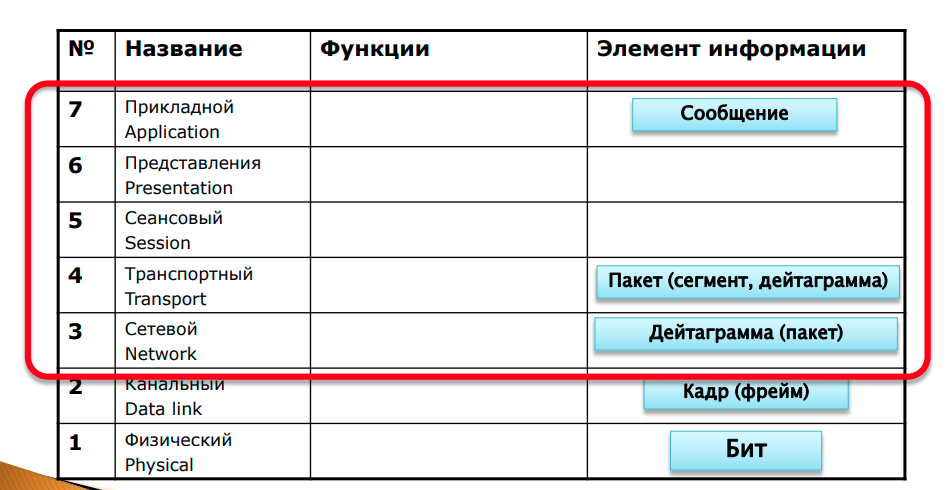
\includegraphics[width=15cm]{images/00/01}
\end{figure}

Иногда под физическим уровнем рисуют физическую среду, а над прикладным приложение/пользователя.

Эта стандартизация позволяет сравнивать между собой разные архитектуры и понимать, что за протокол используется и какая у него функциональная нагрузка.

\begin{enumerate}

\item Физический уровень позволяет соединить между собой два устройства и передать минимальную единицу информации~--- бит. Обычно объединён с канальным уровнем и говорят про протоколы канльного-физического уровня.

\item Канальный объединяет между собой элементы компьютерной сети и позволяет двум узлам, находящимся в одной компьютерной сети обмениваться между собой потоками информации. Элемент информации~--- кадр (фрейм). Это последовательность бит, которая реализует канальный протокол. На канальном уровне могут обмениваться информацией только устройства, непосредственно соединённые канальной средой (проводной/оптической или беспроводной). То есть устройства видят друг друга без посредников. 

Примеры протоколов канального уровня: 
\begin{itemize}
    \item Ethernet (IEEE 802.3)
    \item Wi-Fi (IEEE 802.11)
\end{itemize}

\item Сетевой уровень предназначен для обмена информацией в многосегментной сети, где два конкретных узла могут быть не связаны между собой. Единица информации~--- дейтаграмма (пакет). Здесь реализуется функция адресации. Не обеспечивает никакой надёжности.

Примеры протоколов сетевого уровня:
\begin{itemize}
    \item IPv4
    \item IPv6
    \item ICMP
\end{itemize}

\item Транспортный уровень отвечает за транспортировку информации между приложениями. Раньше говорили про связь между узлами, а сейчас о конкретных приложениях. Здесь реализуется функция аддресации приложений. Он обеспечивает определённый уровень надёжности транспортировки данных от одного приложения к другому. Элемент информации~--- пакет (иногда называют сегмент, иногда дейтаграмма).

Примеры протоколов транспортного уровня:
\begin{itemize}
    \item TCP
    \item UDP
\end{itemize}

\item Сеансовый уровень ко всемы предыдущему добавляет возможность установления и разрыва логического канала между двумя участниками соединения. Специального названия у элемента информации нет. Если как-то и называют, то просто пакетом.

\item Уровень представления предназначен для согласования формата и кодировок информации с двух сторон. Например, общие алгоритмы сжатия информации, общие алгоритмы кодирования, представление в национальных языках. Обычно протоколов уровня исполнения в последнее время не бывает, а если и бывает, то элемент информации~--- пакет.

\item Прикладной уровень~--- реализация конкретных прикладных функций. Передача файла, передача электронной почты... Элемент информации~--- либо пакет, либо сообщение.

Примеры прикладных протоколов:
\begin{itemize}
    \item HTTP
    \item FTP
    \item ...
\end{itemize}

\end{enumerate}

Мы не будем заниматься 3-7 уровнями. 1 и 2 уровни реализуются аппаратно. 3-7~--- программно.

\Subsection{Архитектуры компьютерных сетей}

\begin{itemize}
    \item DNA (DECNet). В 80-90 годы была одной из доминирующих на рынке локальных и корпоративных компьютерных сетей. Проиграла TCP/IP
    \item SNA. Архитектура мейнфреймов в IBM. До сих пор используется в IBM. Имеет коннекты к TCP/IP. Широко не используется.
    \item DARPA (TCP/IP, Internet). Архитектура американского министерства обороны. 
    \item Novell Netware. Раньше была монополистом в области локальных сетей. Тоже проиграла TCP/IP
    \item SMB. Частично используется в сервисах верхнего (транспортный и выше) уровня. В Microsoft и IBM используется для общего доступа к ресурсам
    \item AppleTalk. <<Сейчас имеет историческое значение>>
    \item XNS (читается зи эн эс). От компании Xerox
    \item IPv6. Ответвление от DARPA. Прекрасный интернет будущего
\end{itemize}

Изучать будем DARPA и IPv6. 

\Subsection{Характеристики архитектур компьютерных сетей}

\begin{enumerate}
    \item Иерархия протоколов. Показывает то, как архитектура устроена, как протоколы взаимодействуют между собой
    \item Соответствие модели ISO. 
    \item Адресация
    \begin{enumerate}
        \item Узлов
        \begin{enumerate}
            \item Индивидуальная (один адрес $\leftrightarrow$ 1 компьютер/сетевой интерфейс)
            \item Групповая (один адрес $\rightarrow$ несколько узлов)
            \item Широковещательная (один адрес $\rightarrow$ все адреса какого-то подмножества сети)
        \end{enumerate}
        В IPv4 есть все три, в IPv6 широковещательная реализована через групповую
        \item Приложений
    \end{enumerate}
    \item Связь с канальным уровнем. Нужно оборачивать пакеты сетевой среды в кадры канальной среды. Для этого есть разные механизмы.
    \begin{enumerate}
        \item Разрешение адресов (мапа адресов сетевого уровня на адреса канального уровня). Протокол, позволяющий запрашивать MAC адрес и прочее~--- это как раз про это
        \item Фрагментация. В сетевом и канальном уровне есть ограничения на размеры пакета/кадра. Эти ограничения бывают разными. Поэтому иногда надо большие пакеты сетевого нарезать в маленькие кадры канльного.
        \begin{enumerate}
            \item Поузловая. Каждый узел, получив пакет, сам занимается фрагментацией
            \item На источнике. С самого начала делим на маленькие кусочки
        \end{enumerate}
        В IPv4 используется поузловая. А в IPv6 на источнике.  
    \end{enumerate}
    \item Сетевые протоколы. Основа любой архитектуры
    \item Маршрутизация. Доставка пакета через сложную сеть от одного узла к другому
    \begin{enumerate}
        \item По типу маршрута
        \begin{enumerate}
            \item Индивидуальная (когда доставляем одному узлу)
            \item Групповая (когда доставляем группе)
        \end{enumerate}
        В IPv4 и то, и то
        \item По адаптивности изменения в сети
        \begin{enumerate}
            \item Статическая (каждый маршрутизатор знает что делать с каждым пакетом)
            \item Динамическая (на лету решаем, что делать с пакетом)
            \item Предопределённая (<<от источника>>) (весь маршрут пакета задаётся на источнике)
        \end{enumerate}
        В IPv4 и IPv6 статическа и динамическая. Для тестирования можно и предопределённую.
        \item По месту проведения маршрутных вычислений
        \begin{enumerate}
            \item Централизованная (есть один узел, который принимает решения о том, как доставлять, по всем маршуртам)
            \item Децентрализованная (каждый решает сам)
            \item Гибридная
        \end{enumerate}
        В сетях TCP/IP децентрализованная и гибридная. Централизованная используется в неком <<ныне популярном>> SDN
        \item По числу возможных маршрутов
        \begin{enumerate}
            \item Однопутевые (на одну сеть сохраняется один маршрут)
            \item Многопутевые (на одну сеть несколько маршрутов)
        \end{enumerate}
        В TCP/IP в основном однопутевые, но есть несколько многопутевых протоколов.
        \item По характеру используемой информации для принятия решения
        \begin{enumerate}
            \item Глобальные (нужно знать топологию всей сети)
            \item Локальные (знаем информацию о соседях)
            \item Смешанные (знаем о соседях и ещё о какой-то части сети)
        \end{enumerate}
        В TCP/IP локальные и смешанные
    \end{enumerate}
    \item Транспортные механизмы
    \begin{enumerate}
        \item Дейтаграммные. Транспортировка путём посылки дейтаграмм без гарантии поставки и времени порядка их прихода
        \item Потоковые. Гарантия доставки, сохранение последовательности передачи пакетов
        \item Многопоточные. Между приложениями несколько потоков. Внутри каждого потока гарантии как у потокового
    \end{enumerate}
    В TCP/IP дейтаграммный это UDP, потоковый~--- TCP. Есть SCTP. Не получил широкого распространения, но это многопоточный и входит в TCP/IP
    \item Именование ресурсов
    \item По типу маршрута. Мнемонические имена, которые используются, чтобы людям было удобнее работать
    \begin{enumerate}
        \item Одноуровневое
        \item Двухуровневое
        \item Иерархическое
    \end{enumerate}   
    В TCP/IP иерархическая (spb.hse.ru)
    \item Прикладные протоколы
    \begin{enumerate}
        \item Удалённый терминал
        \item Передача файлов
        \item Электронная почта
        \item ...
    \end{enumerate}
    \item Управление
    \item Защита информации
\end{enumerate}

Изучив эти 11 характеристик, можно понять, как работает архитектура. Мы будем изучать всё это про DARPA.

\Subsection{История создания}

В 1957 создали организацию DARPA при минстерстве обороны.

В 1968 там создали сеть ARPANET.

В 1969 впервые передали данные между двумя университетами. По легенде, один послал другому 1 байт, после чего оба зависли.

В 1974 разработали TCP/IP. 

В 1983 ARPANET перешёл с NCP на TCP/IP.

В 1984 создали DNS.

1989~--- создание WWW и первой версии HTTP.

В 1990 приняли единый термин Internet (вместо ARPANET).

1993~--- первый браузер Mosaic.


\begin{figure}[H]
  \centering
  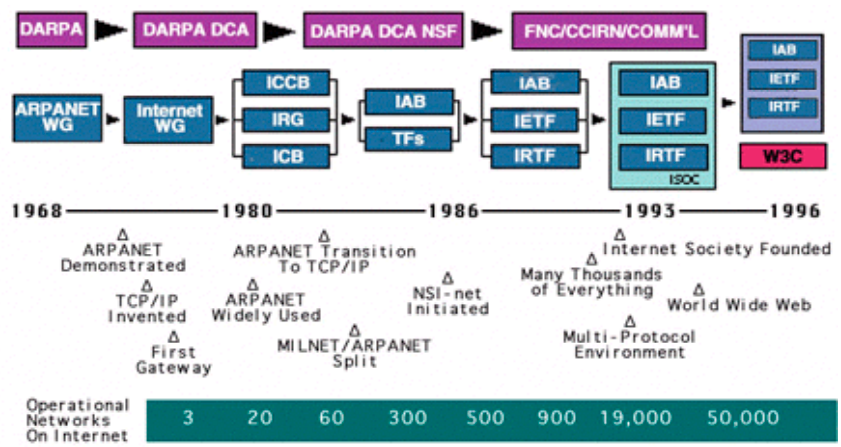
\includegraphics[width=15cm]{images/00/02}
\end{figure}

\Subsection{Стандартизирующие организации Internet}


Internet Society (ISOC)~--- сообщество, занимающееся развитием Internet
\begin{enumerate}
    \item Internet Architecture Board (IAB)~--- координирует развитие TCP/IP
    \begin{enumerate}
        \item Internet Engineering Steering Group (IESG)~--- рассмотрение стандартов и технические работы для IETF
        \item Internet Engineering Task Force (IETF)~--- самый главный комитет. Выпускают RFC
        \item Internet Research Task Force (IRTF)~--- развитие технологий, которые могут понадобиться в будущем
        \item Internet Corporation for Assigned Names and Numbers (ICANN)~--- централизованное назначение адресов и номеров (ранее IANA)
    \end{enumerate}
\end{enumerate}

\Subsection{Координирующие организации Internet}

Network Information Center (NIC)~--- организации, ответственные за распределение адресов
\begin{enumerate}
    \item InterNIC~--- США
    \item Reseaux IP Europeens (RIPE)~--- Европа
    \item African Network Information Centre (AfriNIC)~--- Африка
    \item Asia Pacific Network Information Centre (APNIC)~--- Азия
    \item Regional Latin-American and Caribbean IP Address Registry (LACNIC)~--- Латинская Америка
    \item Russian Institute for Public Networks (RIPN)~--- Россия
\end{enumerate}

\Subsection{Стандарты TCP/IP}

Все стандарты TCP/IP~--- это текстовые документы с уникальным номером (RFC). Все они лежат на ietf.org/rfc.html

Там нет жёсткой стандартизации, некторые места можно истолковать двояко, не все им следуют.

Сначала их делили на FYI и STD. В последнее время так не делают

\Subsection{Иерархия протоколов TCP/IP}

\begin{figure}[H]
  \centering
  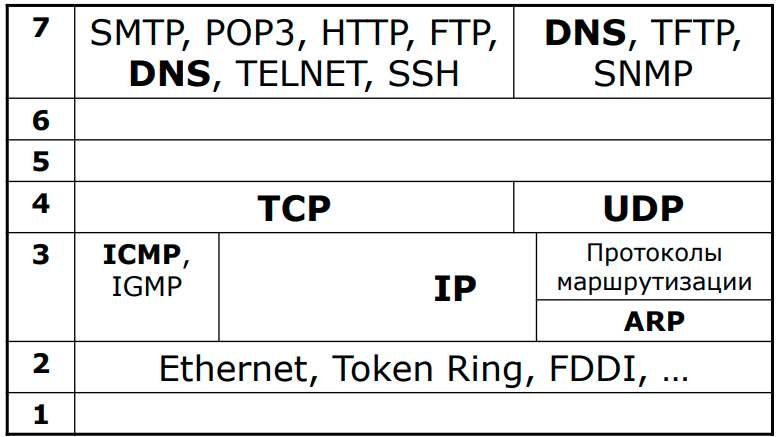
\includegraphics[width=15cm]{images/00/03}
\end{figure}

Самым важным протоколом является протокол сетевого уровня IP. На сетевом уровне находятся также ICMP (протокол управляющих сообщений, расширяет собой IP) и IGMP (протокол групповых сообщений), ARP (связь с канальным уровнем), огромное число протоколов маршрутизации.

На транспортном уровне TCP и UDP. 

На сеансовом уровне и уровне представления протоколов нет, поскольку кусок роли установления сеанса выполняет TCP (в UDP сеанса вообще нет). В TCP/IP шестого уровня нет. То есть каждый раз реализуем представительский протокол. Это жутко неудобно, привело к куче проблем и это архитектурная ошибка.

На прикладном уровне миллион разных протоколов. Слева транспорт TCP, справа~--- UDP. 
